Pour une expérience optimale, vous pouvez changer la langue de l’application.

Pour choisir quelle langue utiliser, cliquez sur le bouton “Réglages” (Voir Capture \ref{fig:access-settings}).

\begin{figure}[H]
	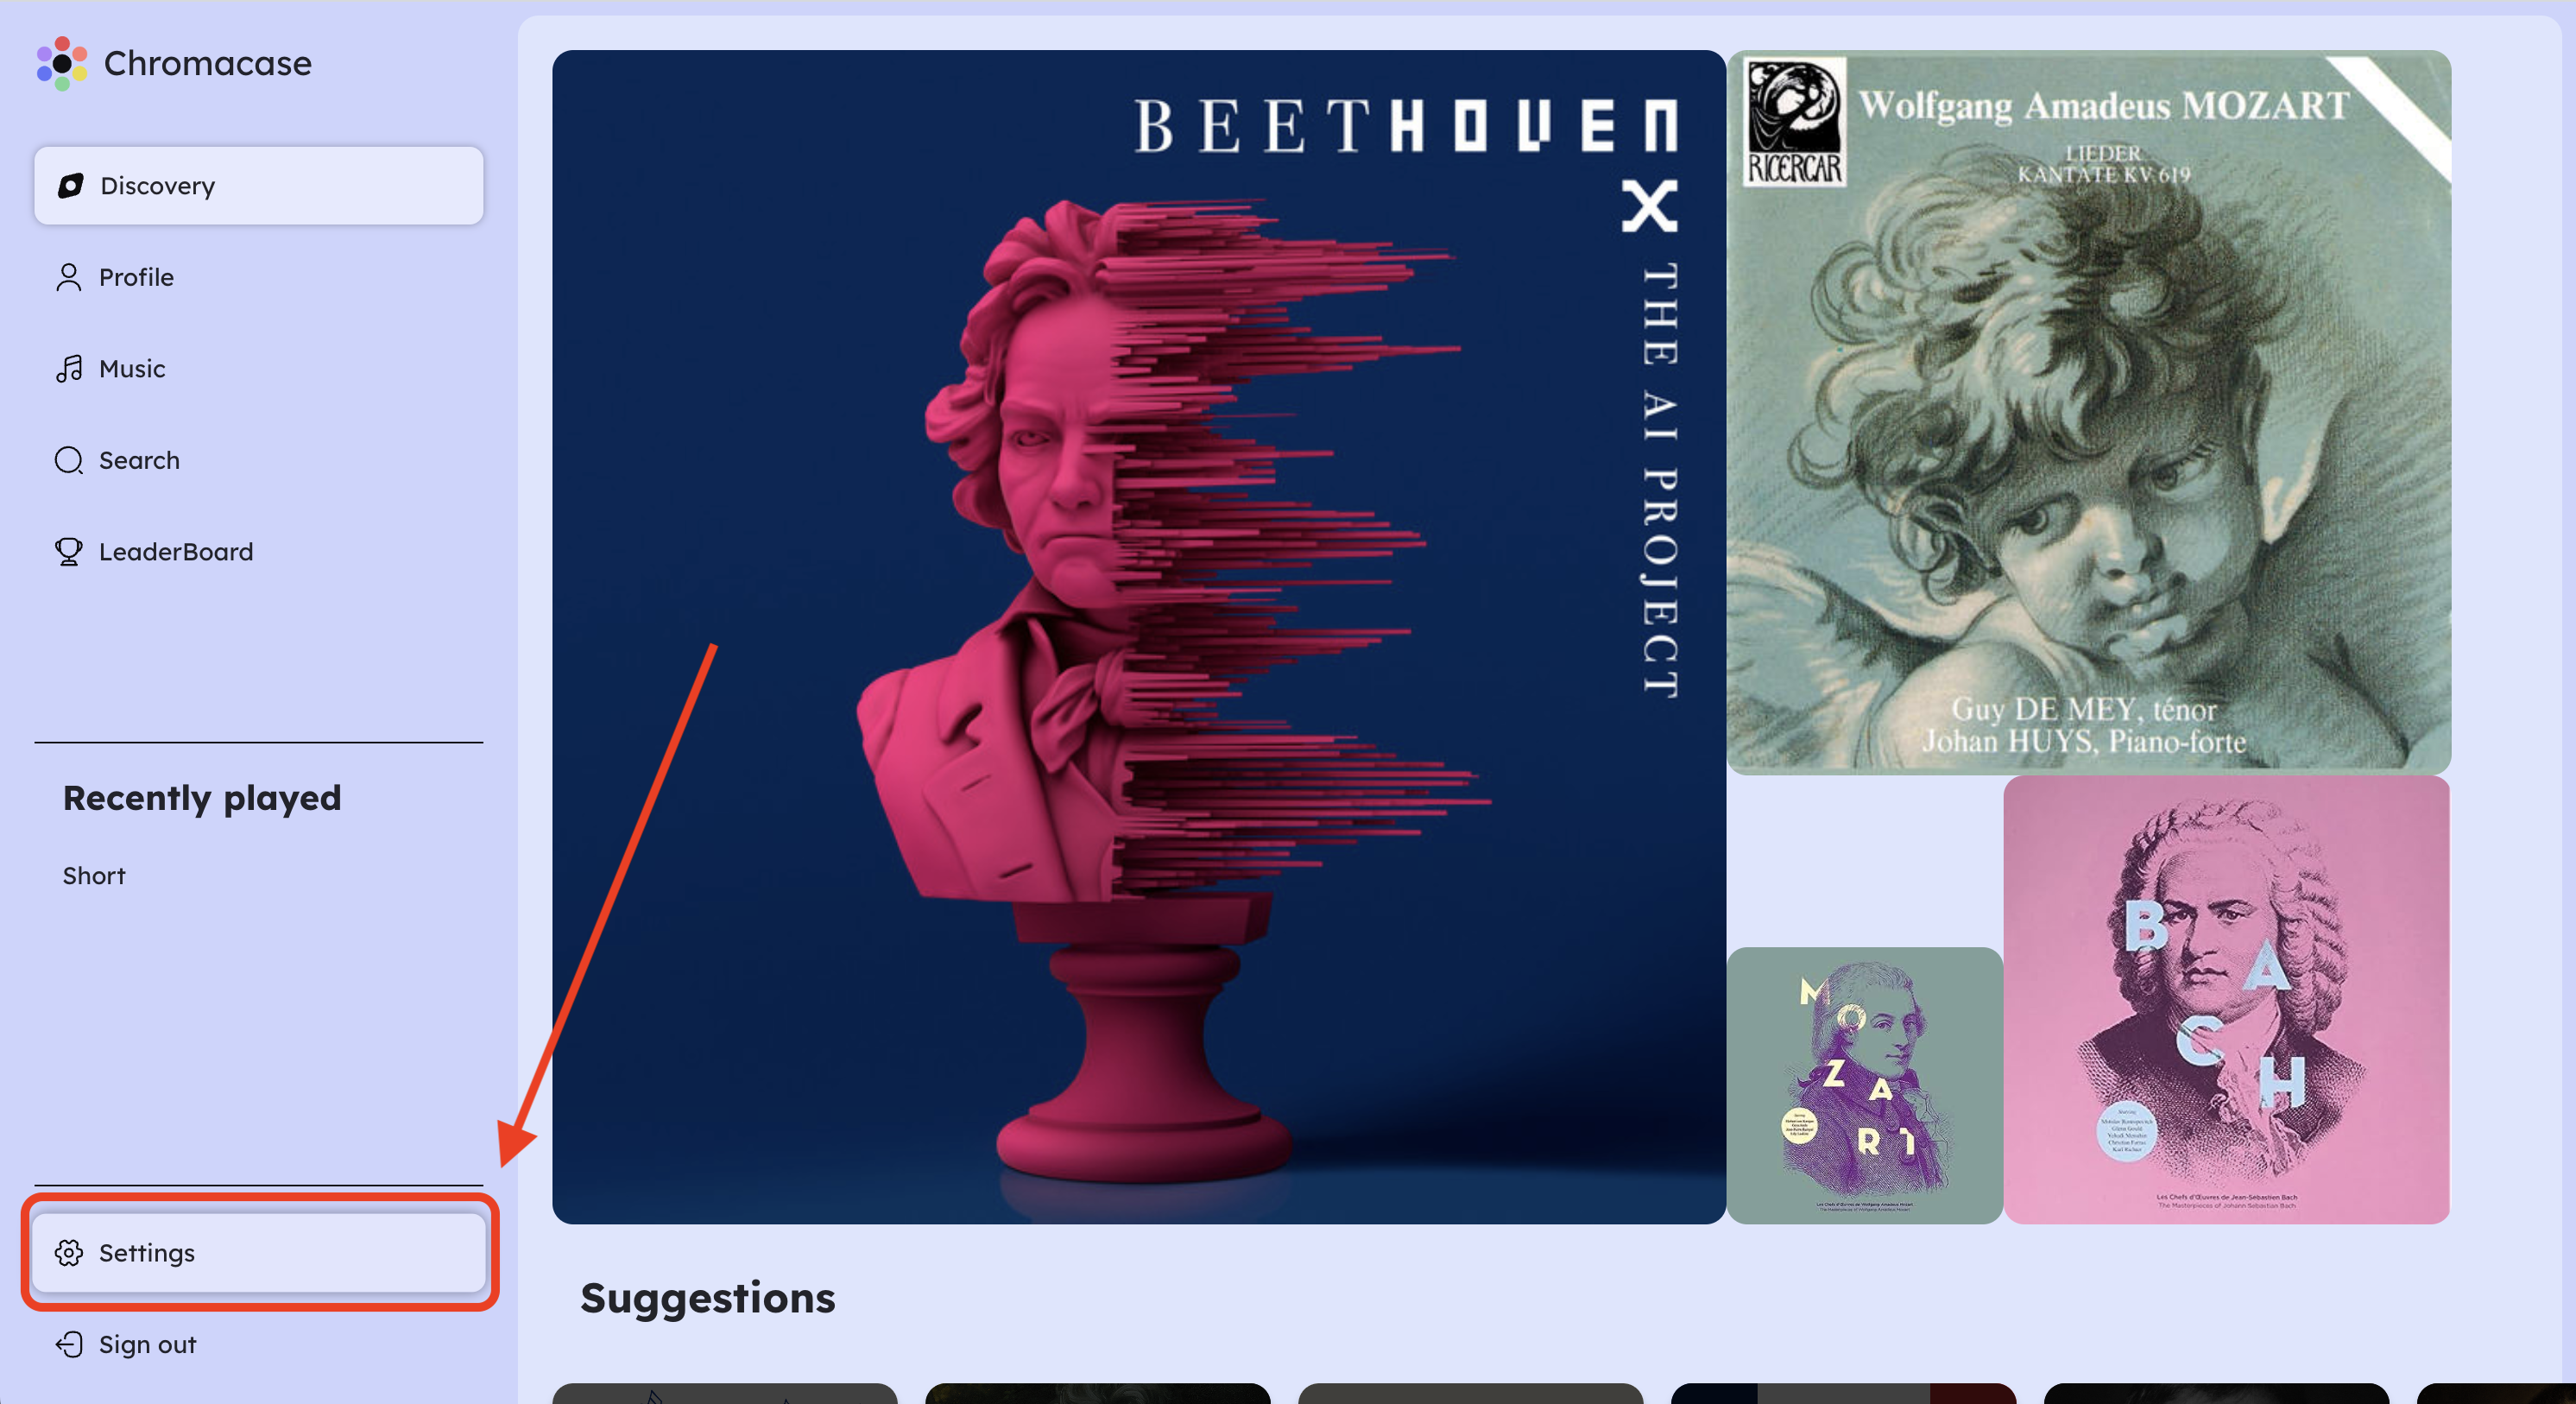
\includegraphics[width=\linewidth]{../\dir/guide/settings/access-settings.png}
	\caption{Acceder aux reglages}
	\label{fig:access-settings}
\end{figure}

Sélectionnez l’onglet “Préférences”, et choisissez l’option de langue à utiliser (Voir Capture \ref{fig:change-language}).

\begin{figure}[H]
	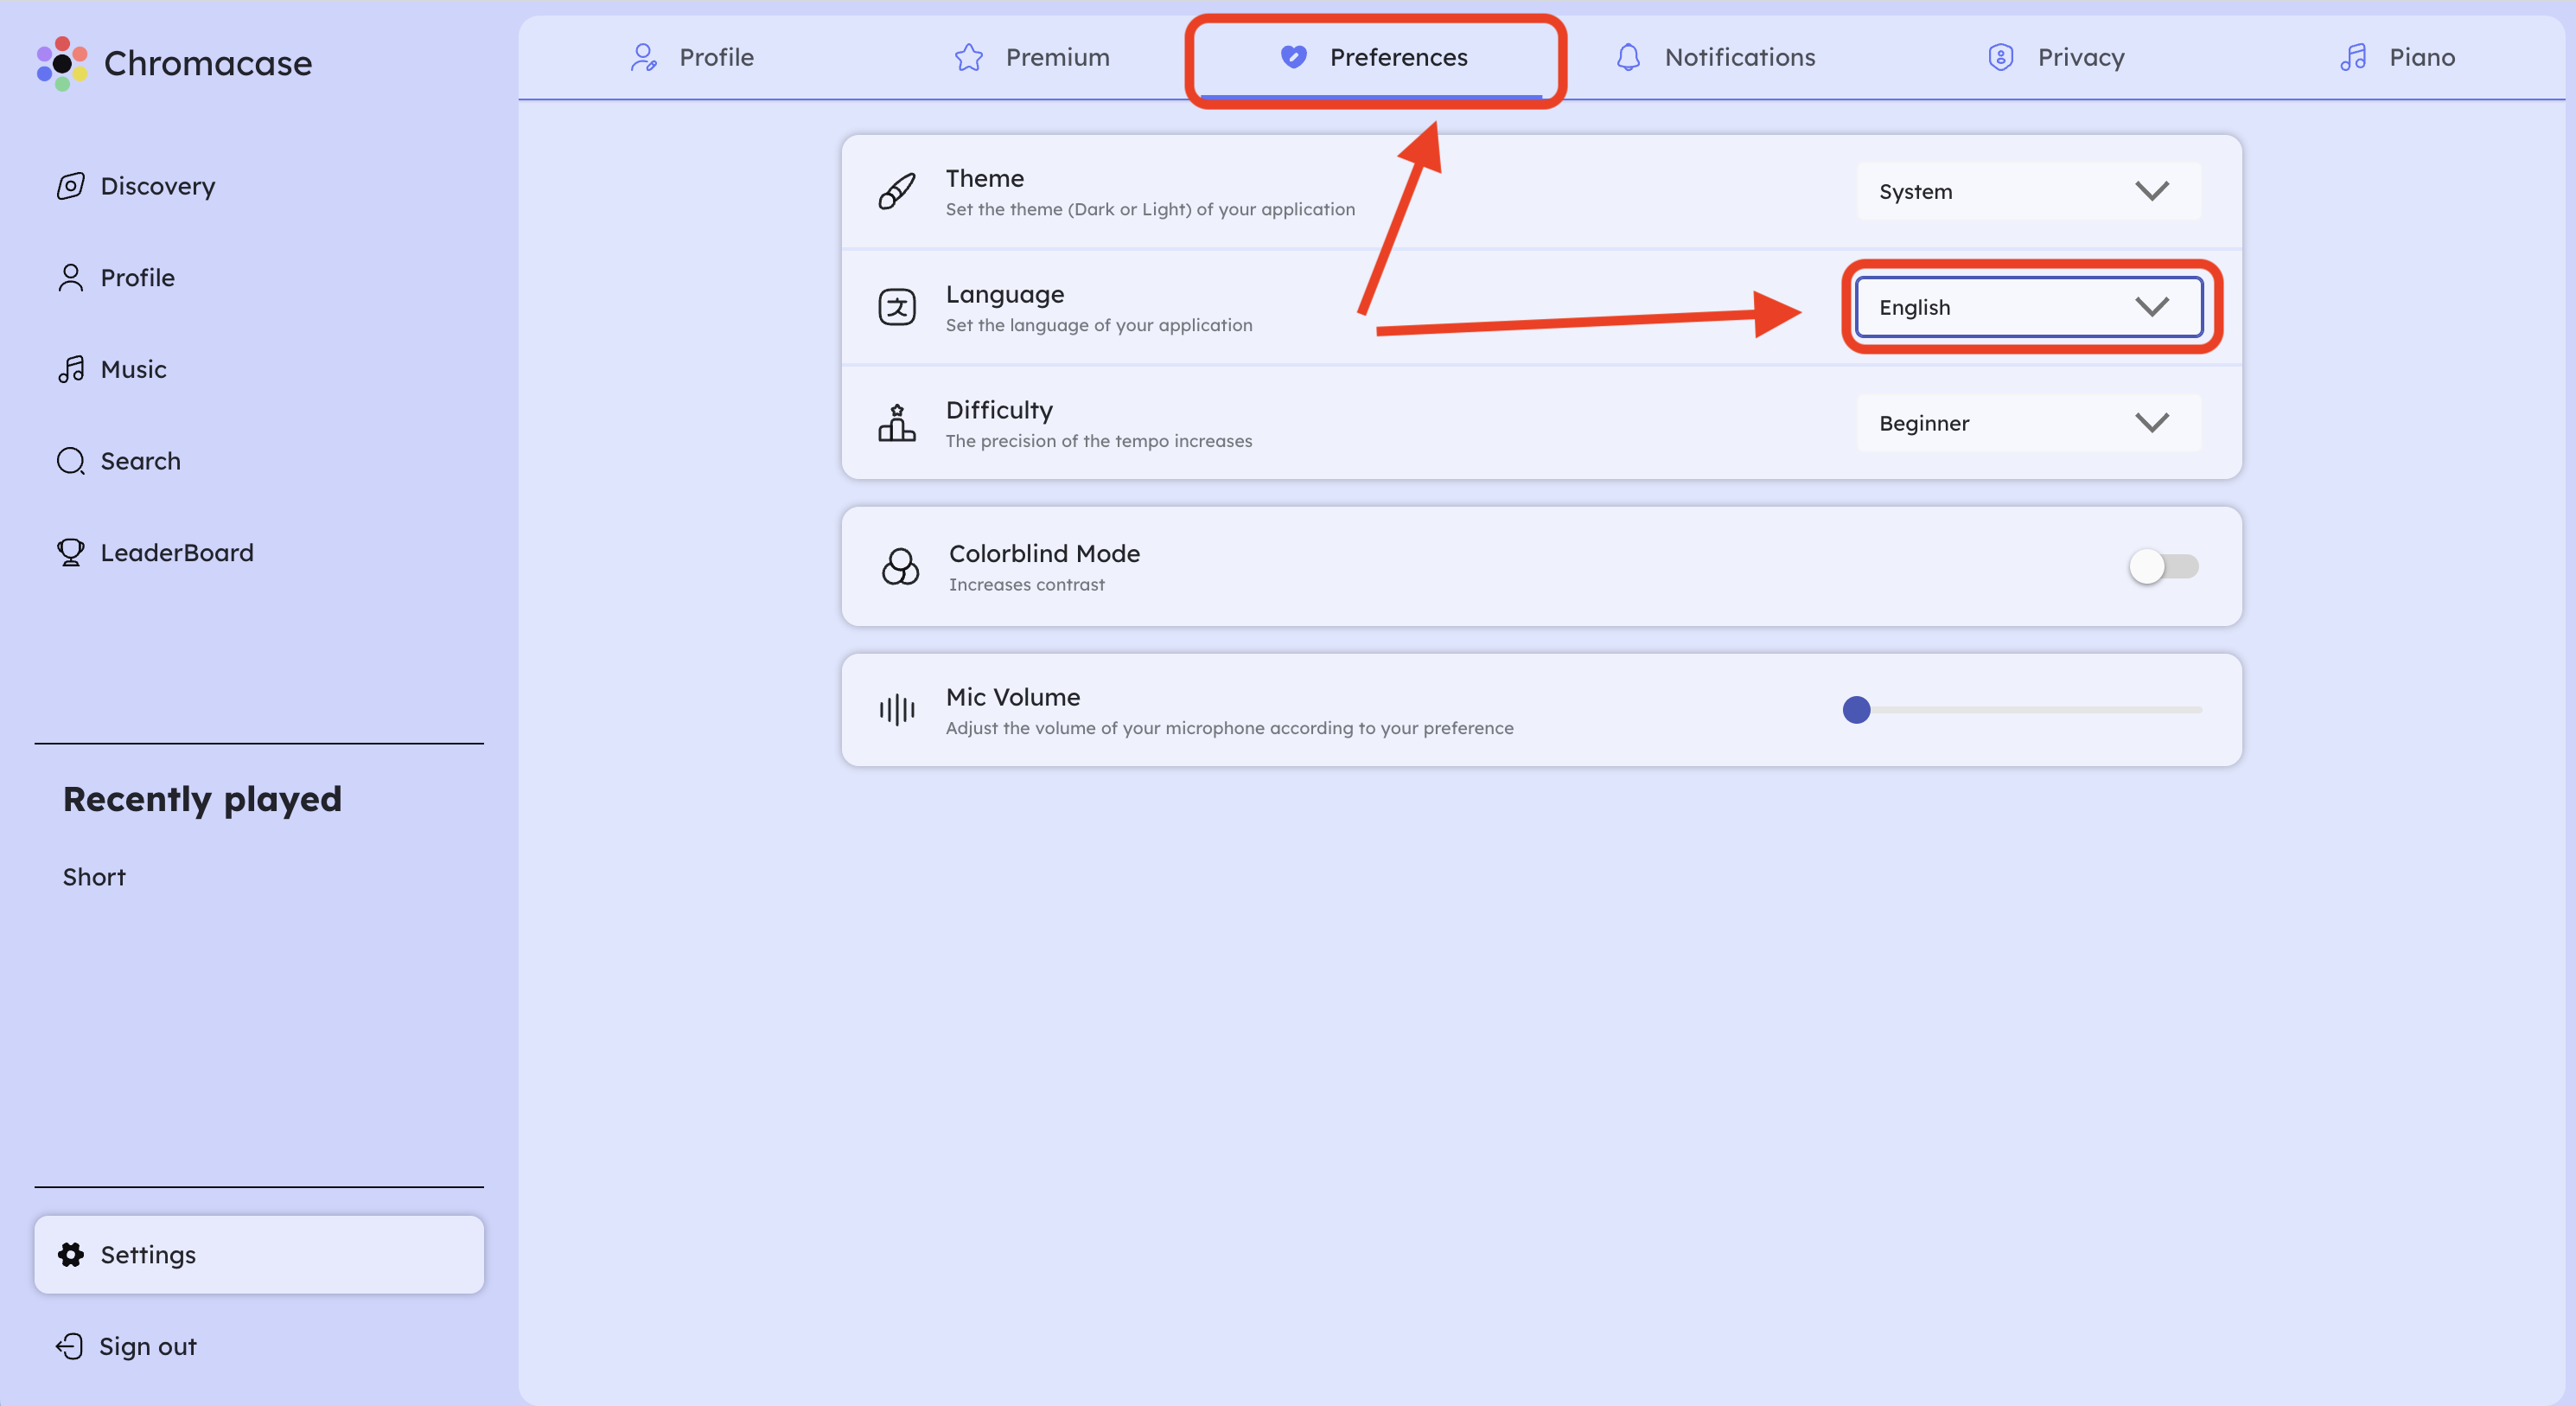
\includegraphics[width=\linewidth]{../\dir/guide/settings/change-language.png}
	\caption{Selectionner la langue}
	\label{fig:change-language}
\end{figure}
